% Appendix Template

\chapter{Rigid Body Transformation} % Main appendix title

\label{AppendixB} % Change X to a consecutive letter; for referencing this appendix elsewhere, use \ref{AppendixX}

\lhead{Appendix B. \emph{Rigid Body Transformation}} % Change X to a consecutive letter; this is for the header on each page - perhaps a shortened title

	\emph{Rigid body} is the one in which distance between any two given points on it remains constant in time regardless of external forces exerted on it. Rigid body transformation forms the basic components in the pose detection framework. In this appendix we give the key ideas behind the rigid body transformations. We consider a $3D$ operational space represented by the vector space $\Re^3$. We consider a right-handed reference frame with homogenous dimensions along each axes. In $\Re^3$, a rigid body is represented by \emph{6 degrees of freedom (DOF)}, 3 for the position along each of the coordinate axes (cartesian coordinates) $P = [p_x,p_y,p_z]^{\text{T}}$ and 3 for the orientation $R$. Considering the system shown in the Figure~\ref{fig:frame_ref} below where $F_0$ is the world frame and $F_1$ is the frame attached to the rigid body. Suppose we know the position $^{1}P$ in the frame $F_1$ and let $^{0}O_1$ be the relative displacement of $F_1$ with respect to $F_0$. Given this framework, the position $^{0}P$ can be given by using the \emph{Homogenous Transformation Matrix}: $^{0}T_1$.
	
\begin{wrapfigure}{r}{0.5\textwidth}
\begin{center}
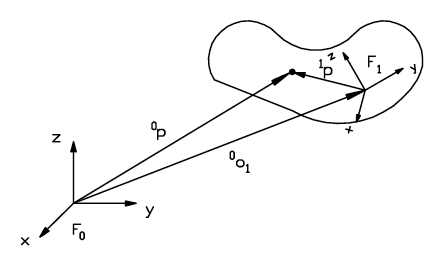
\includegraphics[width=0.5\textwidth]{assets/rigid_body.png}
\end{center}
\caption{Rigid body transformation}
\label{fig:frame_ref}
\end{wrapfigure}

\begin{align*}
^{0}T_1 = \begin{bmatrix}
^{0}R_1 & ^{0}O_1 \\
0_{1\times 3} & 1
\end{bmatrix}
=
\begin{bmatrix}
n_x & s_x & a_x & o_x \\
n_y & s_y & a_y & o_y \\
n_z & s_z & a_z & o_z \\
0 & 0 & 0 & 1 \\
\end{bmatrix}
\end{align*}


where $^{0}R_1$ is the direction cosine matrix describing the rotation of the frame $F_1$ with respect to $F_0$. $^{0}R_1$ is an orthonormal matrix so ideally 3-DOF is enough for the representation of the orientation. A quick look of the different representation of orientation is presented in Table~\ref{table:rotation} 

\begin{table}

\end{table}